\section{Hardware} \label{sec:hardware-devel}
This section will focus on presenting how the different hardware pieces have been integrated between themselves and, ocasionally, explain difficulties that have been encountered during the process.
The proposed hardware structure of the slave device that was previously presented can be visualised in \autoref{fig:connection_diagram}.

Some GPIO pins of the Raspberry Pi can provide alternative functionality other than a General Purpose IO pin (GPIO), such as serving as a pin to access an SPI communication channel.
The Raspberry Pi pins 17 and 18 have been chosen to interface with encoder signals because they do not provide any alternative functionality, they are true GPIO pins.
This way, no alternative functionality that could potentially be useful in future works is occupied by the encoder interface.

We have also used a 7.5V power supply to provide power to the DFR0592, which in turn will drive the motor.
The criteria was to use a value supported by both equipment, and 7.5V fits both the DFR0592 range (7-12V) and the DC motor range (6-9V)

\begin{figure}[htp]
	\centering
	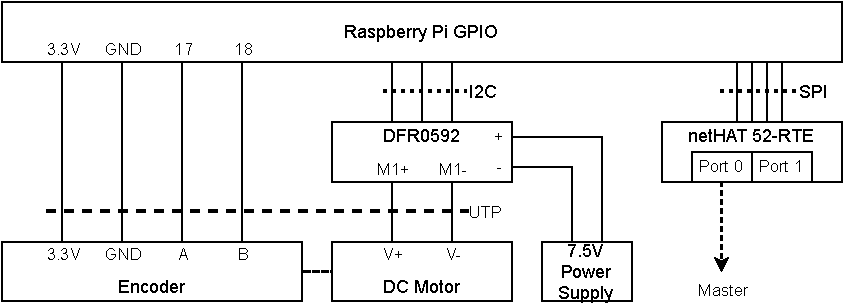
\includegraphics[width=0.8\textwidth]{connection_diagram.pdf}
	\caption{Hardware connection diagram of the proposed slave device}
	\label{fig:connection_diagram}
\end{figure}

% Motor Assembly
% `- Encoder soldering
% `- Cable soldering
% `- Magnetic disc attachment
\subsection{Motor assembly}
We began working on the hardware implementation by assembling the motor parts, which require some soldering.
First we soldered the encoder board on the motor terminals, being careful to leave enough motor shaft length available to be able to attach the encoder's magnetic disc on it.
Then we proceeded to solder a 6-wire cable to the encoder board terminals, which export all necessary electrical connections.

The exported connections are the encoder power supply ($VCC$ and $GND$, assigned to the blue/white-blue wire pair), the encoder output signals ($A$ and $B$, assigned to the green/white-green wire pair) and the motor power signals ($M1$ and $M2$, assigned to the orange/white-orange wire pair) and they can be visualised on \autoref{fig:encoder_board}.
A generic 8-wire Ethernet UTP cable was used for the above mentioned electrical connections.
These cables are fairly inexpensive and can provide the necessary power to the DC motor.
Finally we attached the magnetic disc on the motor shaft so the encoder can work as expected.

\begin{figure}[htp]
	\centering
	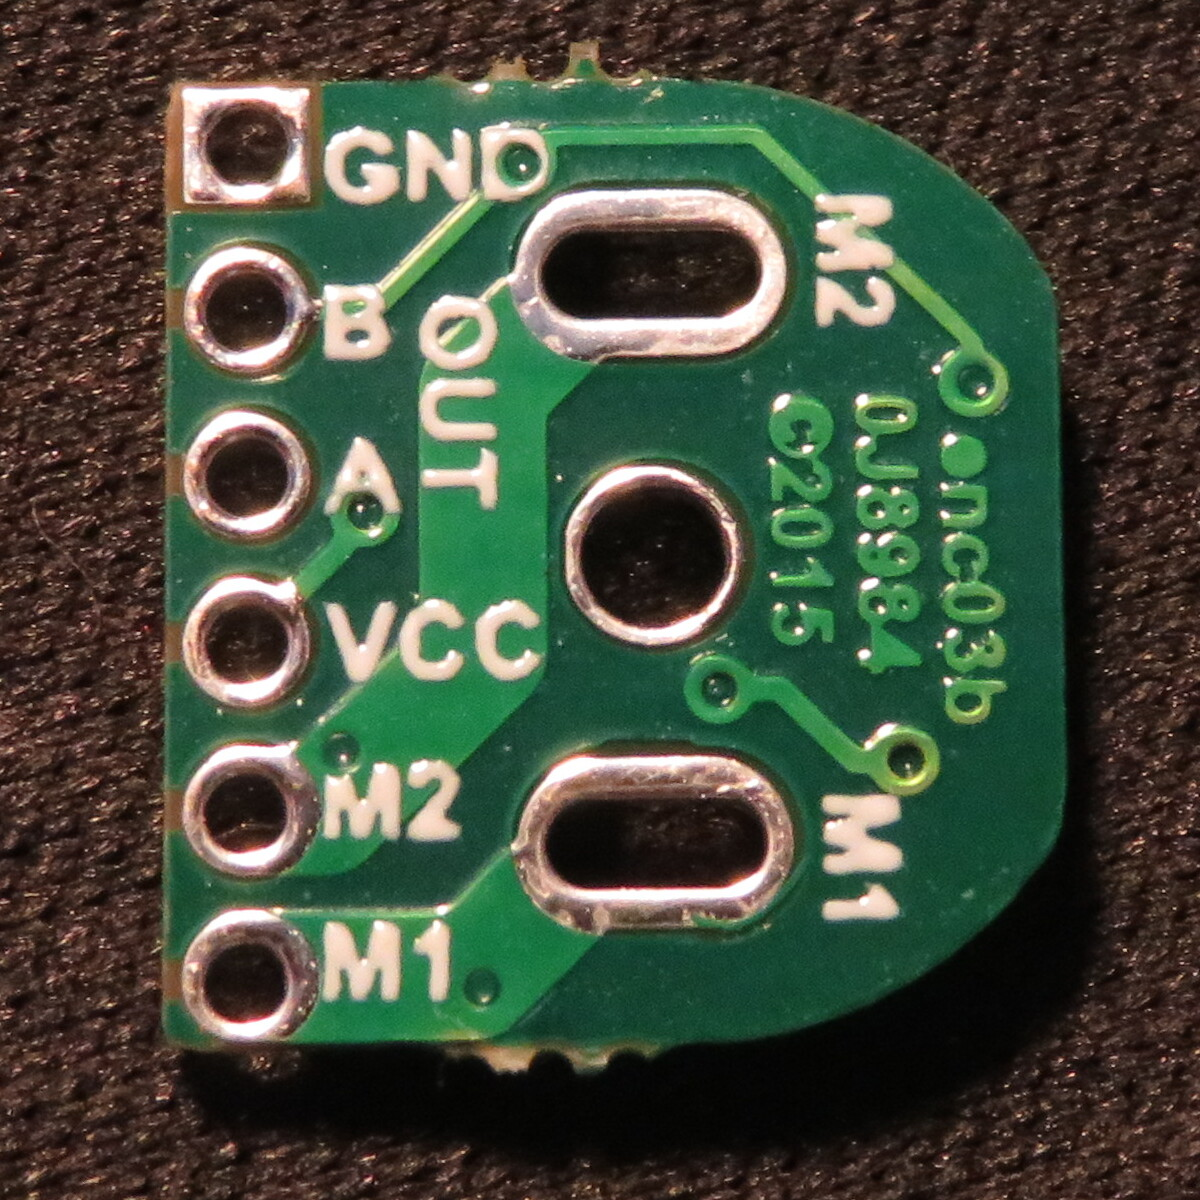
\includegraphics[width=0.8\textwidth]{encoder_board.JPG}
	\caption{Motor encoder board connections}
	\label{fig:encoder_board}
\end{figure}

% Motor Support
% `- 3D design
% `- 3D printing
% `- Adding the motor
\subsection{Motor support}
In order to not let the motor lay down on a table, a simple 2-piece support was designed to give it form and stability.
We also included a disc in the design to act as a minimalist load for the motor.
A preview of the designed pieces can be seen on \autoref{fig:support_base}, \autoref{fig:support_arc} and \autoref{fig:support_disc}.
The CAD design was developed in Blender \cite{sw:blender} and the three drawn pieces were then exported to STL format.
Finally these three STL files were sent to a 3D printing service to be printed.
The final result of the assembled motor coupled with the support can be seen in \autoref{fig:final_motor_stage}.

\begin{figure}[htp]
	\centering
	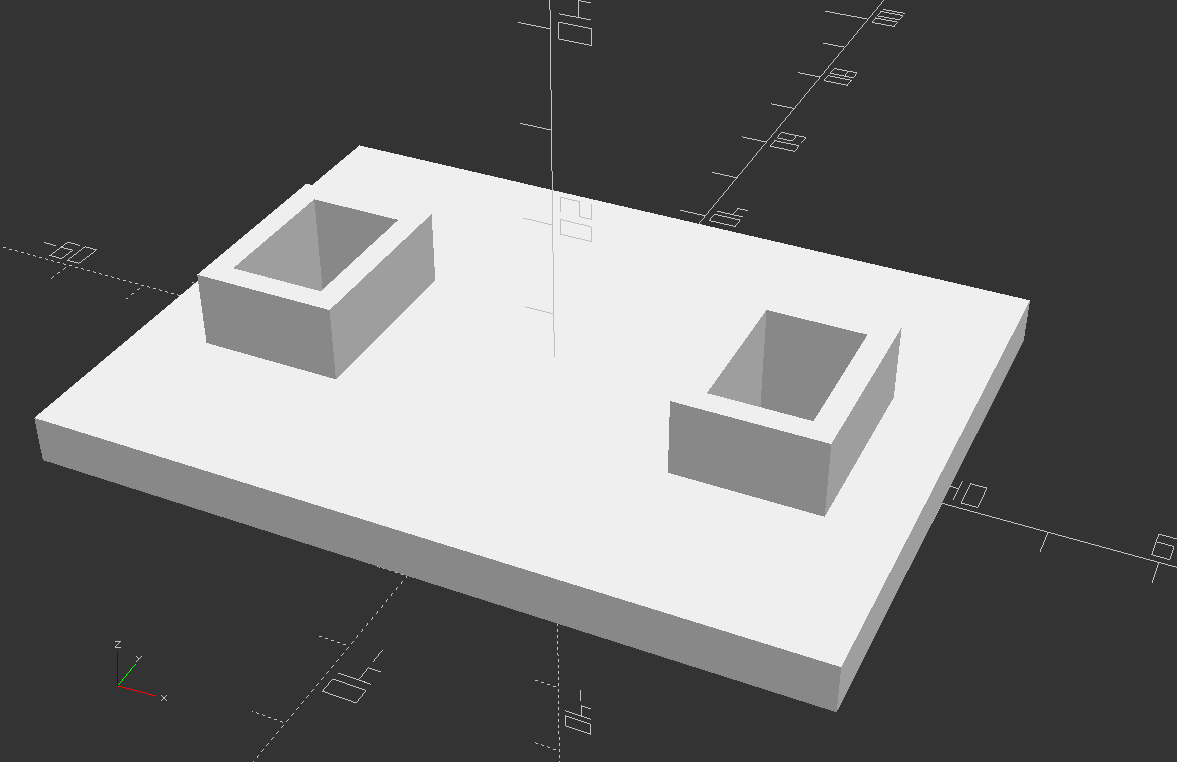
\includegraphics[width=0.8\linewidth]{base.png}
	\caption{Support foot preview}
	\label{fig:support_base}
\end{figure}
\begin{figure}[htp]
	\centering
	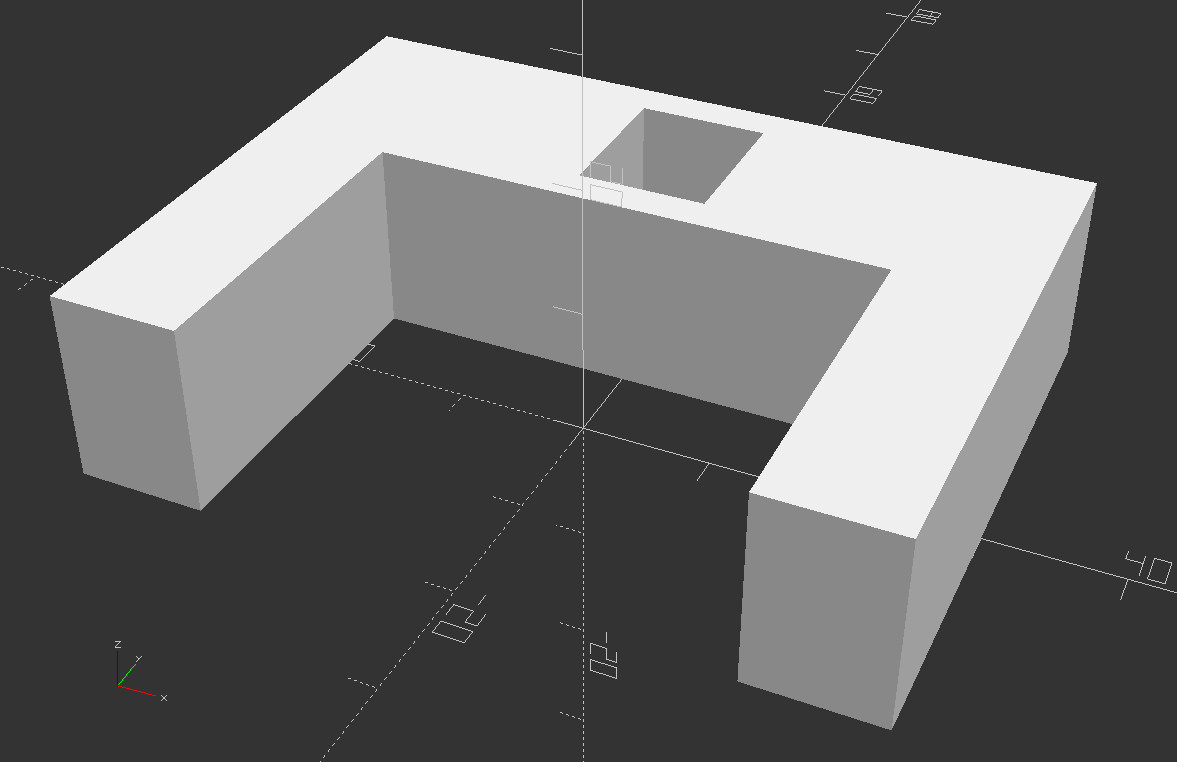
\includegraphics[width=0.8\linewidth]{suporte.png}
	\caption{Support arc preview}
	\label{fig:support_arc}
\end{figure}
\begin{figure}[htp]
	\centering
	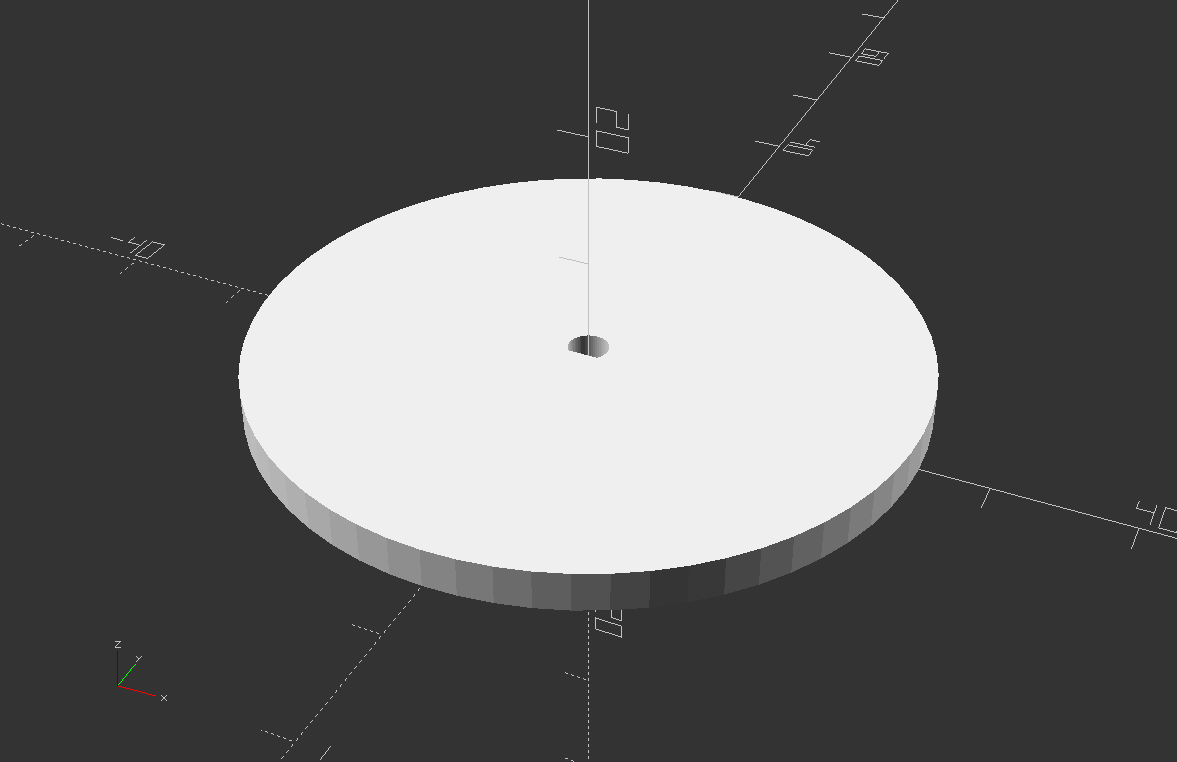
\includegraphics[width=0.8\linewidth]{disco.png}
	\caption{Motor disc preview}
	\label{fig:support_disc}
\end{figure}
\begin{figure}[htp]
	\centering
	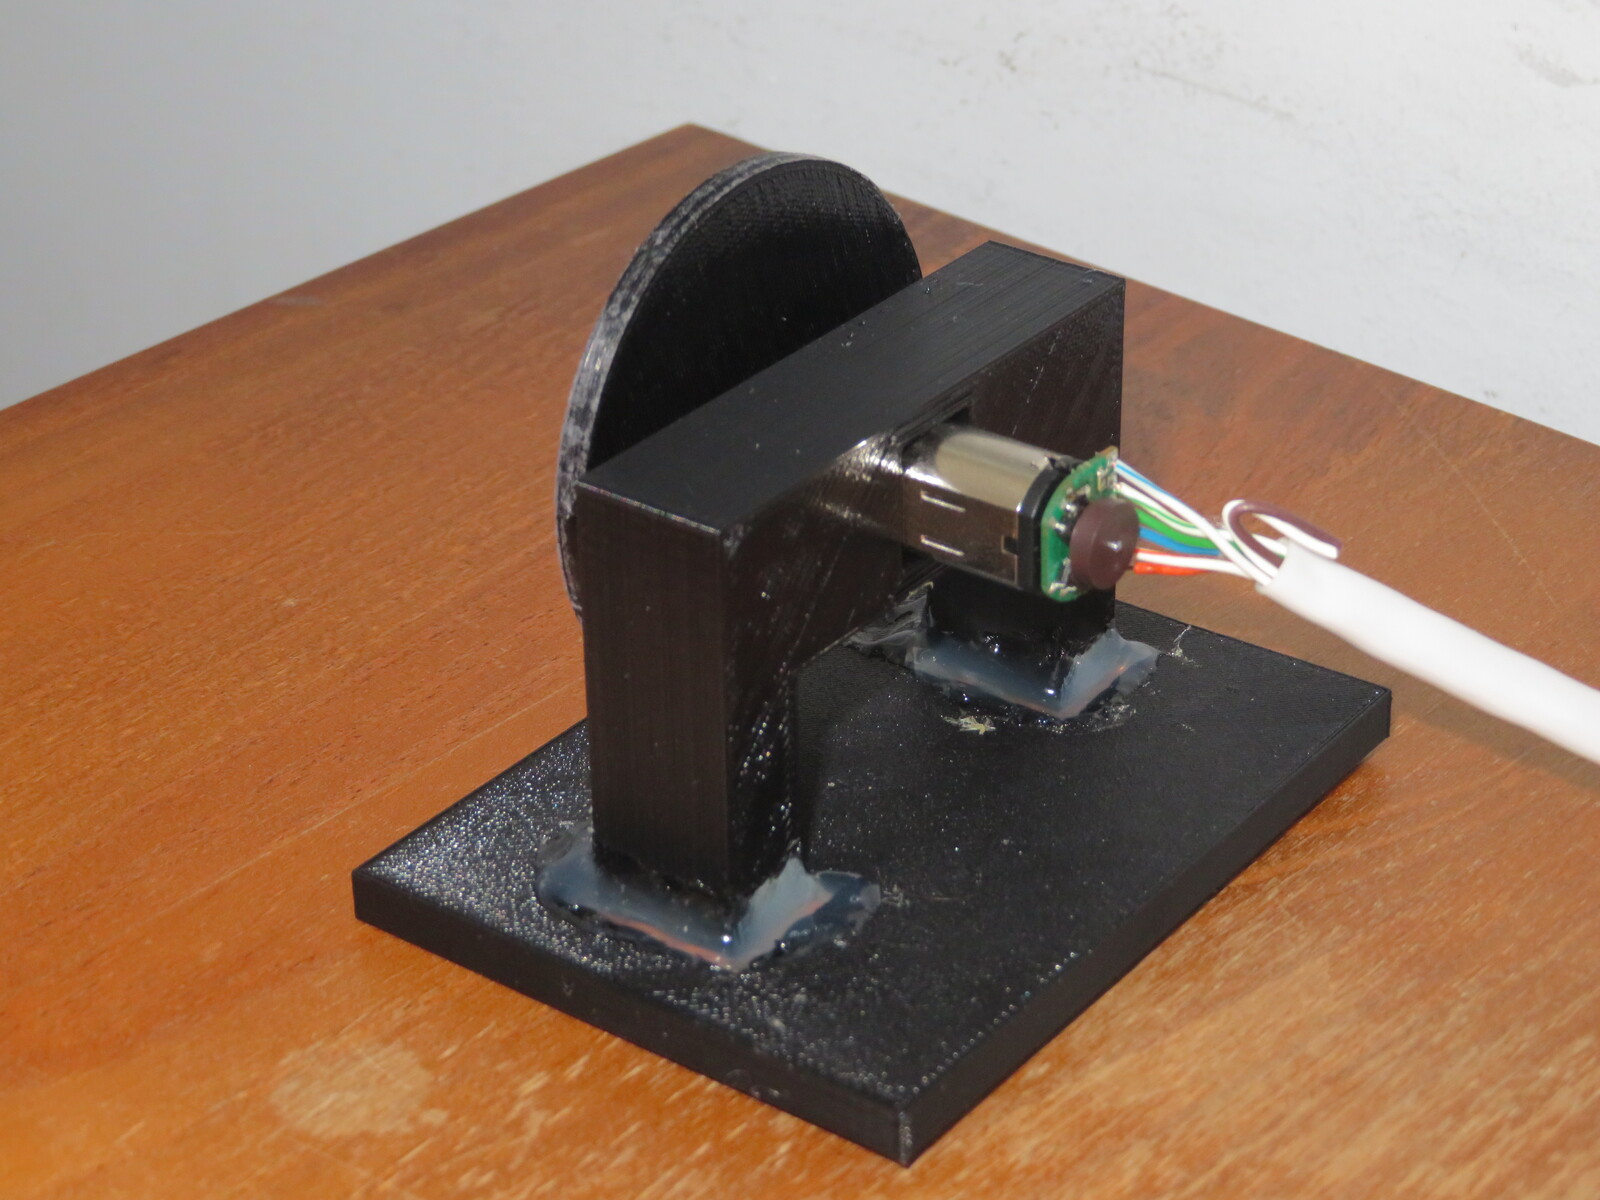
\includegraphics[width=0.8\linewidth]{IMG_2859_scaled.jpg}
	\caption{Fully assembled motor with support}
	\label{fig:final_motor_stage}
\end{figure}

% Raspberry Pi stack assembly
% `- Raspberry Pi
% `- GPIO exporter
%   `- encoder cables
% `- DFR0592
%   `- PSU cable
% `- netHAT 52-RTE
\subsection{Raspberry Pi stack}

After having obtained the necessary components, we assembled the slave device by stacking the different HAT boards onto the Raspberry Pi 4 board.
The final result can be seen in \autoref{fig:final_rpi_stack}.
Having done it for the first time we considered the boards to have an unstable mechanical coupling, so we added a series of hexagonal spacers and screws to give the entire stack a bit more rigidity and robustness.

\begin{figure}[htp]
	\centering
	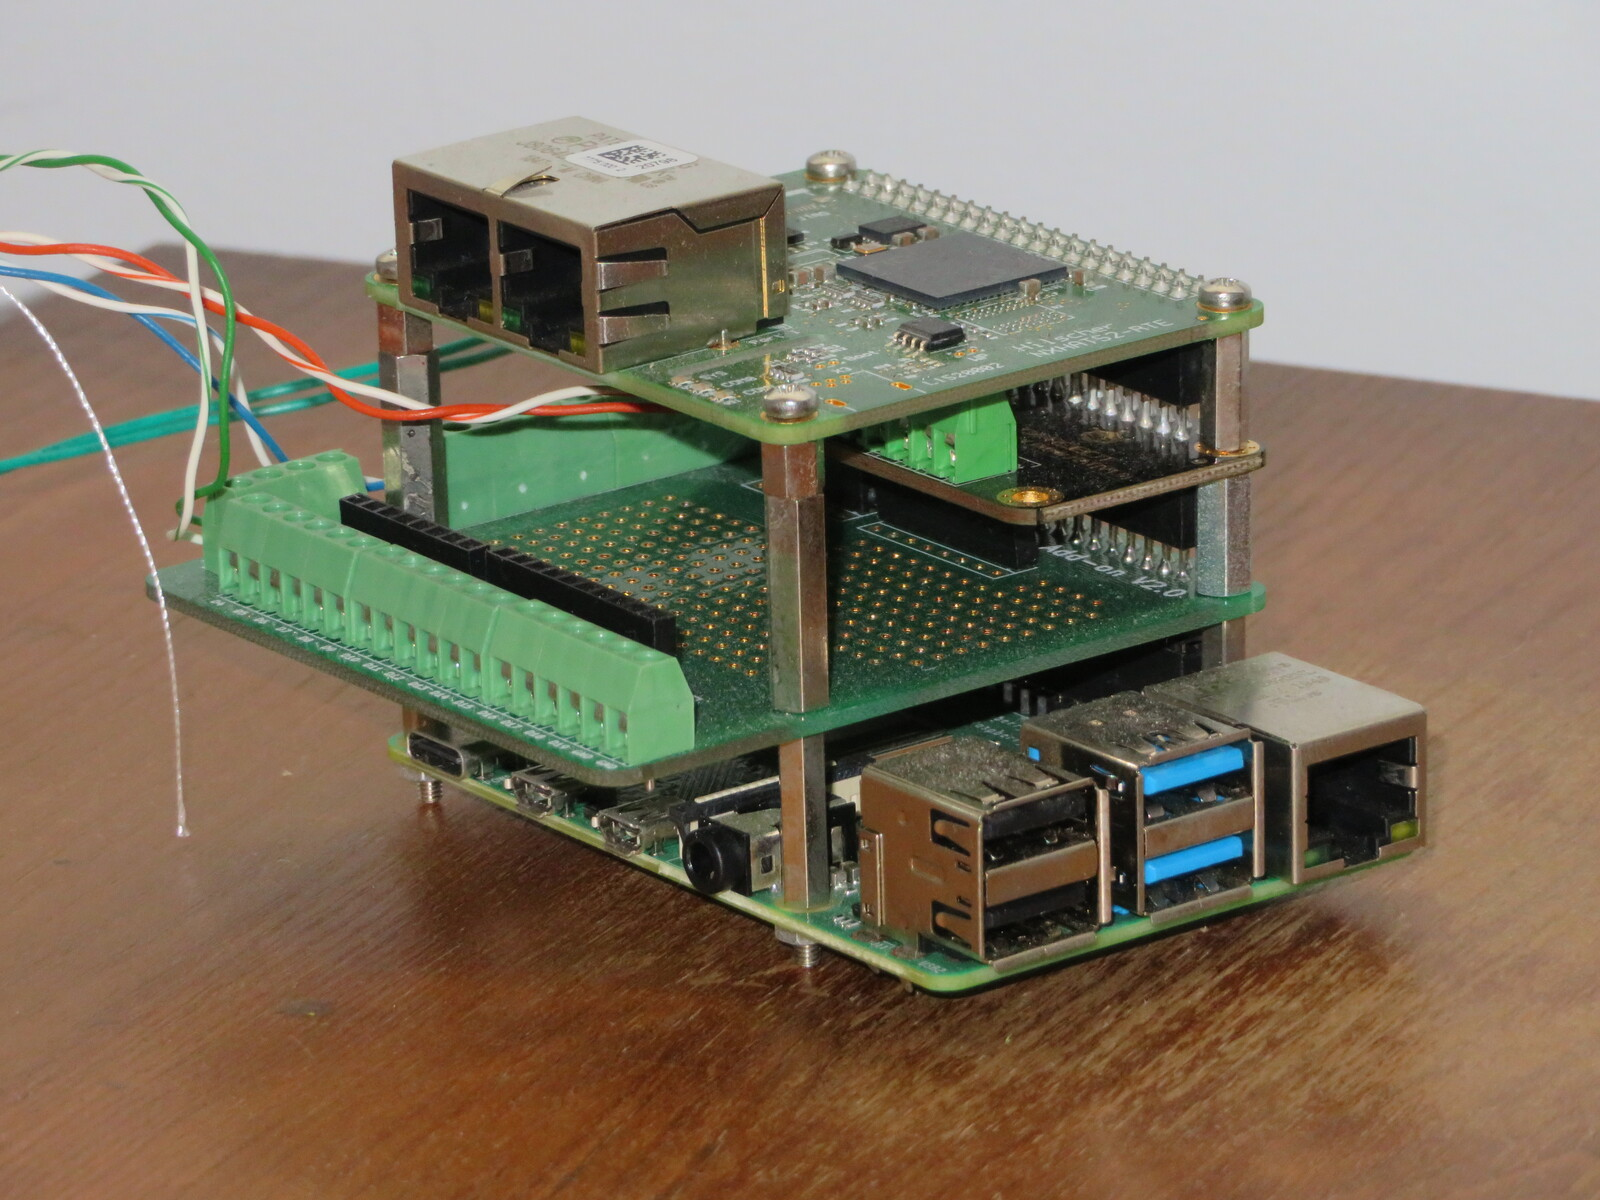
\includegraphics[width=0.8\linewidth]{IMG_3040_resized.JPG}
	\caption{Fully assembled Raspberry Pi stack}
	\label{fig:final_rpi_stack}
\end{figure}

The full stack is comprised of:
\begin{enumerate}
	\item a Raspberry Pi 4 board \cite{product:rpi4} on the bottom, followed by;
	\item a generic screw terminal prototype board that exports the GPIO signals to the screw terminals, useful to connect the encoder signals to the GPIO pins (at the time of writting, the specific board used has been discontinued);
	\item the DFR0592 motor interface board;
	\item and, on the top of the stack, the Hilscher's netHAT 52-RTE board, which comes with a non-passthrough GPIO connector, forcing it to be placed on the top.
\end{enumerate}

\subsection*{Final result}

\begin{figure}[htp]
	\centering
	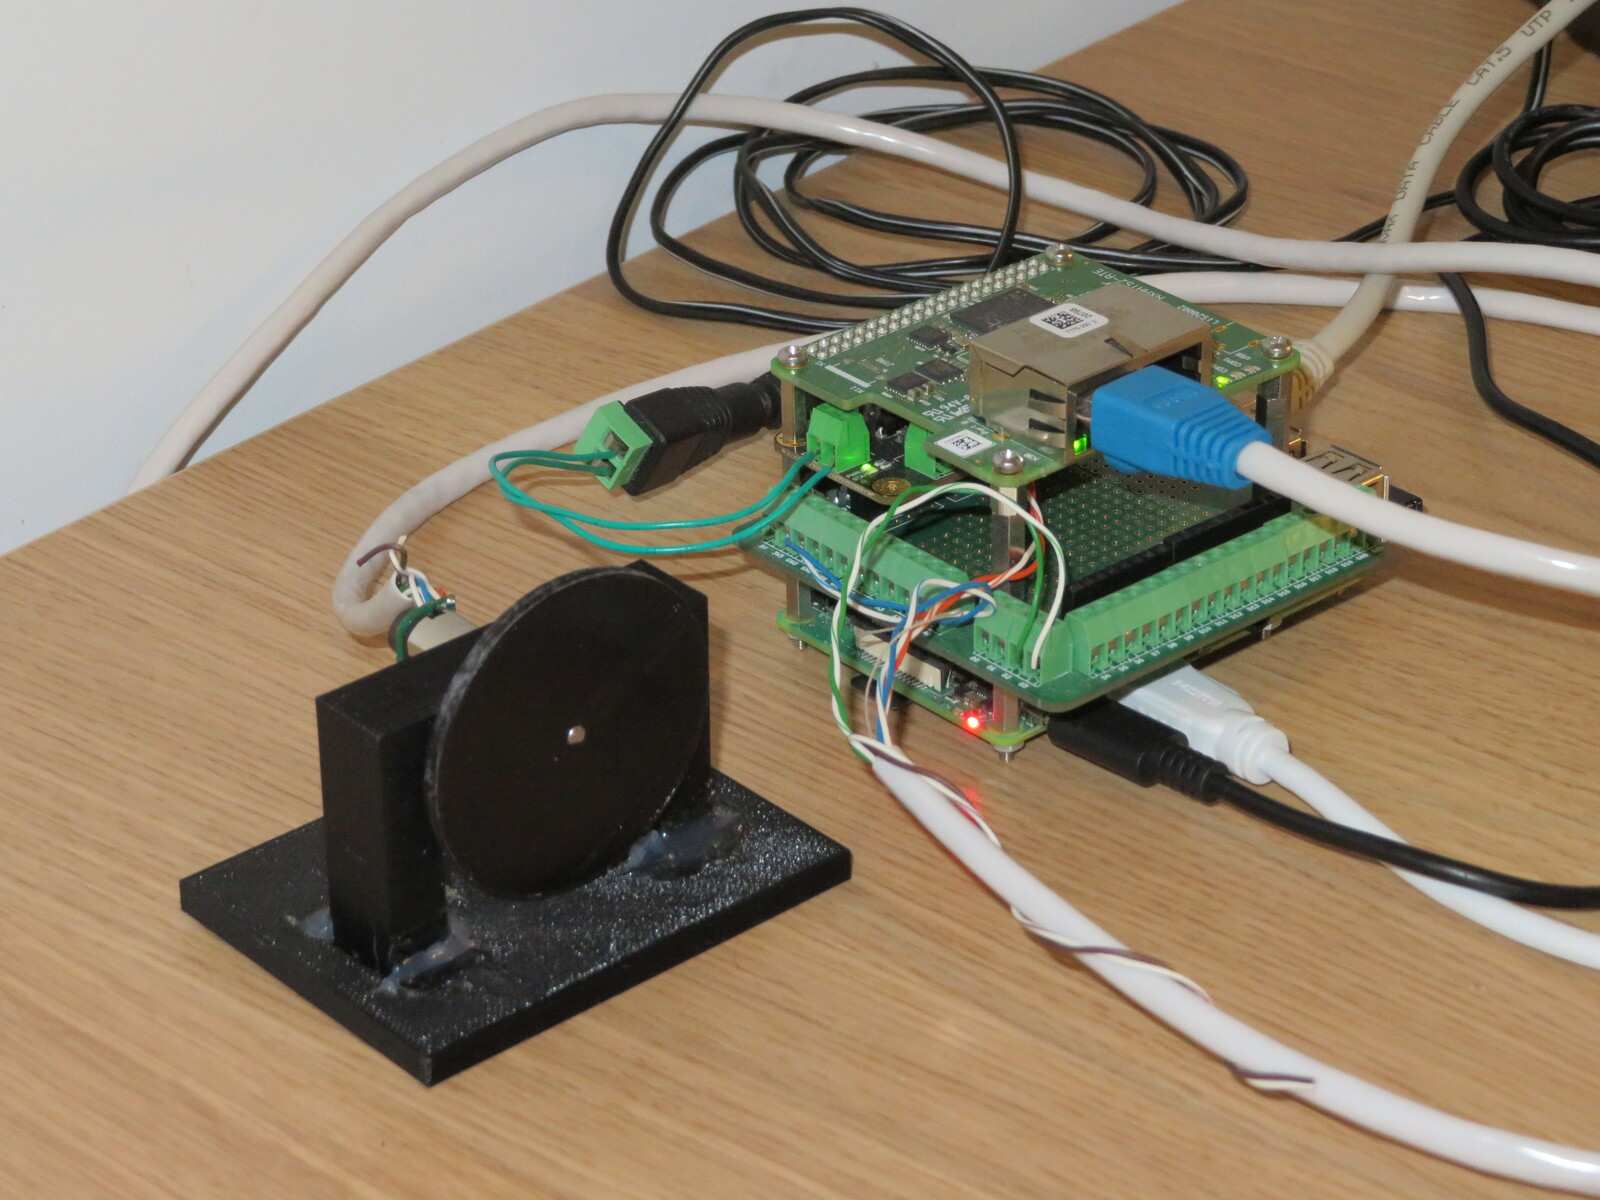
\includegraphics[width=0.8\linewidth]{hardware_overview.JPG}
	\caption{Overview of the entire slave device hardware}
	\label{fig:hardware_overview}
\end{figure}
